\section{Preliminaries}
\label{sectionmodel}

%Connectivity model			#lebhar2009unit

In this section, we describe system model of an energy-restricted large-scale network, and we formulate the Neighbor Discovery problem formally.
The notations are listed in Table \ref{notations}.

\begin{table}[!t]
\renewcommand{\arraystretch}{1.3}
\caption{Notations for Neighbor Discovery}
\label{notations}
\centering
\scalebox{0.92}{
\begin{tabular}{|c|c|}
\hline
\bfseries Notation & \bfseries Description\\
\hline
$N$ & The number of nodes in the network\\
\hline
$u_i$ & node $u_i$ with ID $i$ \\
\hline
$u_{ij}$ & the $j^{th}$ neighbor of node $u_i$ \\
\hline
$\delta_{ij}$ & The transmission time drift between $u_i$ and $u_j$ \\
\hline
$n*$ & The average number of neighbors is $n$, $n=p_nN$ \\
\hline
$t_0$ & The length of a time slot \\
\hline
$L(i,j)$ & The discovery latency that node $u_i$ discovers node $u_j$ \\
\hline
$L(i)$ & The discovery latency that node $u_i$ discovers all neighbors \\
\hline
$\theta$ & The pre-defined global duty cycle\\
\hline
$\theta_i$ & Node $u_i$'s local duty cycle\\
\hline
$W$ & The time slot spent by a node discovering all neighbors\\
\hline
$M$ & Neighboring matrix, $M_{ij}=1$ means $u_i$ and $u_j$ are neighbors \\
\hline
\end{tabular}}
\end{table}


\subsection{System Model}

We introduce three important factors of an energy-restricted large-scale network.

\textbf{Communication:}
when multiple nodes communicate simultaneously, a transmission may fail due to the communication interference. We adopt the protocol model (also called graph model, unit-disk model\cite{moscibroda2006complexity, wang2015connectivity}) to describe the process, which assumes a node $u_i$ can receive $u_j$'s message successfully if $u_j$ is the only transmitter that is within $u_i$'s communication range.
The protocol model is a popular model that enables the development of efficient algorithms crucial networking problems. Some other models, such as the signal to interference plus noise ratio (\emph{SINR}) model, are more complicated and lack good algorithmic features. In addition, it is shown that these models can be transformed to the protocol model by particular means in \cite{lebhar2009unit}.

\textbf{Network connectivity:}
a node can only discover nodes that are within its communication range under the protocol model. In a large-scale network, two nodes may not be connected directly and we call two nodes connected by one-hop communication as \emph{neighbors}. Thus, a large-scale network is always \emph{partially-connected}, contrary to a fully-connected network in which any two nodes are neighbors, i.e. they are connected by one-hop communication.


\textbf{Energy-restricted:}
a node in the network has very limited energy and we assume a node can turn on or off its radio to save energy. When a node turns on the radio, it can transmit a message including its identifier (ID), or listen on the channel to receive a neighbor's message.

Technically speaking, we assume an energy-restricted large-scale network consisting of $N$ nodes as set $U=\{u_1,u_2,\ldots,u_N\}$.  Nodes are distributed in a large place and they can communicate through a fixed wireless channel. We assume the locations of the nodes obey some distributions, such as uniform distributions and Gaussian distribution\cite{wang2013gaussian}.
Suppose a node has a fixed communication range $\Delta$ and two nodes $u_i, u_j$ are neighbors if their distance suits $d(u_i, u_j) \leq \Delta$. We can use a symmetric matrix $M_{N\times N}$ to represent nodes' neighboring relations as:
$$ M_{i,j}=\left\{
\begin{aligned}
1  & & & & & & {u_i ~and~ u_j ~are~ neighbors}\\
0  & & & & & & {otherwise}\\
\end{aligned}
\right.
$$


Suppose time is divided into slots of equal length $t_0$, which is sufficient to finish a complete communication process (one node transmits a message including its ID and a neighbor receives the message). 
A node who turns its radio on can choose to be transmitting state or listening state:
\begin{itemize}
\item \textbf{Transmitting state:} a node transmits (broadcasts) a package containing its ID on the channel;
\item  \textbf{Listening state:} a node listens on the channel to receive message from neighbors.
\end{itemize}
In the protocol model, a node $u_i$ can discover its neighbor $u_j$ in time slot $t$ if and only if $u_j$ is the only neighbor of $u_i$ that transmits and $u_i$ listens in the slot.

A node has limited energy and it has to turn off the radio to save energy for most of the time. We assume a \emph{duty schedule} for a node $u_i$ is a pre-define sequence $S_i=\{s_i(t)\}_{0\leq t<T}$ of period $T$, in which
$$ s_i^t=\left\{
\begin{aligned}
S  & & & {u_i ~turns~ off~ the~ radio~ in~ slot~ t}  	 \\
T  & & & {u_i ~is~ in~ transmitting~ state~ in~ slot~ t}	\\
L  & & & {u_i ~is~ in~ listening~ state~ in~ slot~ t}	\\
\end{aligned}
\right.
$$
We define \emph{duty cycle} as the fraction of time a node turns its radio on, which is formulated as:
$$\theta_i=\frac{|\{t: 0\leq t<T, s_i(t) \in \{T,L\}\}|}{T}.
$$

If all nodes have the same duty cycle all the time, i.e. $\theta_i = \theta_j$ for any nodes $u_i, u_j$, we call them \emph{symmetric nodes}. Otherwise, they are \emph{asymmetric nodes}. Denote the start time of node $u_i$ as $t_i^s$ and denote $\delta_{ij}$ as the time drift between a pair of neighbors $u_i, u_j$, i.e. $\delta_{ij} = t_i^s - t_j^s$.

\subsection{Problem Definition}

A node $u_i$ executes operations (turning off radio, transmitting, or listening) according to the pre-defined duty schedule $S_i$. 
When $u_i$ starts the neighbor discovery process, denote $L(i,j)$ as the slots cost to find the neighbor $u_j$ and we define \textbf{discovery latency} of node $u_i$ as the time to discover all neighbors:
$$L(i) = \max_{j:M_{i,j}=1} L(i,j).
$$

Note that, neighbor discovery is not bidirectional and any pair of neighbors have to discover each other separately.
We formulate the neighbor discovery problem for node $u_i$ as:
%@@@to be modified
\begin{problem}
For a node $u_i$ and set of its neighbors $N_i = \{u_j | d(u_i, u_j)\leq \Delta \}$, design duty schedules for all nodes such that:
$\forall u_j \in N_i$ :
$$
\begin{aligned}
&\exists t \ s.t. :   \\%\quad 
&s_i(t) = L ,
s_{j}(t) = T, and~
\forall u_k \in N_i, u_k \neq j : s_{k}(t) \in \{L, S\}.
\end{aligned}
$$
\end{problem}
%@@@

\begin{figure}[!h]
\centering
\subfigure[The topology of a simple wireless network]{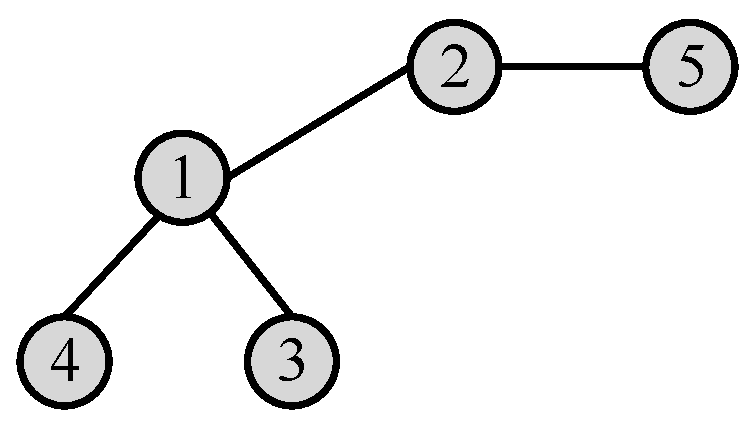
\includegraphics[width=1.65in]{./Figure/topology.eps}}
\vspace{0.03in}
\subfigure[Neighbor discovery process]{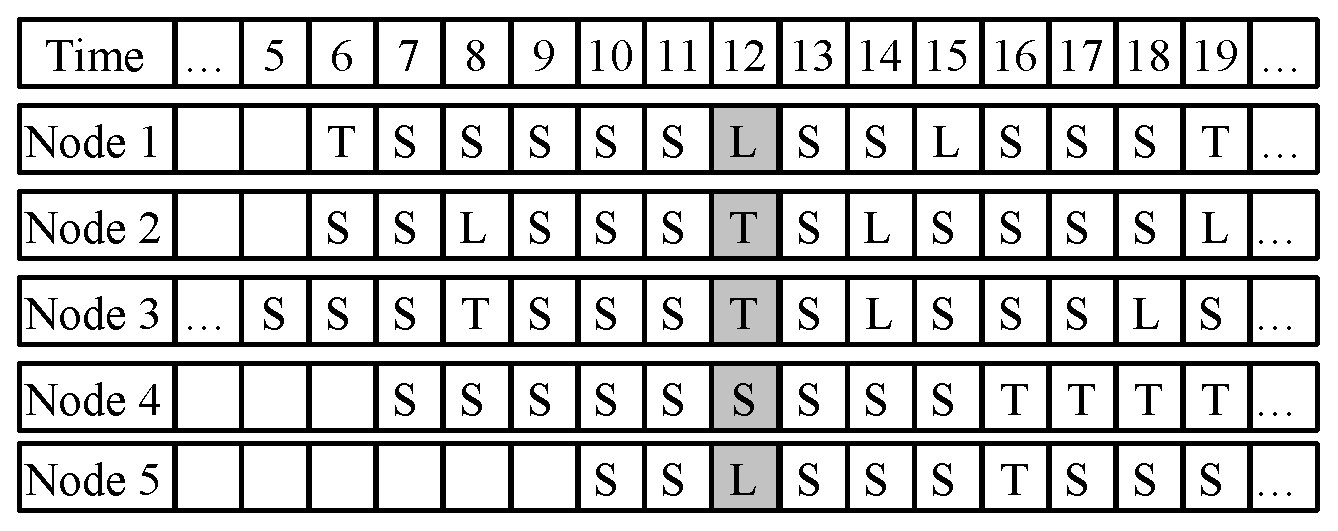
\includegraphics[width=2.8in]{./Figure/NBexample.eps}}
\caption{An example of neighbor discovering process. S, T and L represents Sleep pattern,
Transmitting state and Listening state in wake-up pattern respectively.}
\label{NDexample}
%\vspace{-0.2in}
\end{figure}

Fig.\ref{NDexample} shows an example of $5$ nodes, the topology is depicted in Fig.\ref{NDexample}(a), and Fig.\ref{NDexample}(b) describes the neighbor discovery process. The duty cycle is set as $0.25$ and nodes start in different time slots.
The designed duty schedule for node $u_1$ is $S_1 = \{ T, S, S, S, S, S, T, S, S, T, S, S, S, T, ... \}$.
Suppose time drift between node $u_1$ and $u_4$ is $\delta_{14} = 1$; $u_1$ $u_2$ start in the same time slot. 
In slot $12$, node $u_5$ discovers neighbor $u_2$, but node $u_1$ cannot discover $u_2$ since another neighbor $u_3$ is in transmitting state simultaneously.

%An example of neighbor discovery process is given in Fig.\ref{NDexample}.
%Fig.\ref{NDexample}(a) shows the topology of a simple
%wireless network, which consists of $5$ nodes.
%Fig.\ref{NDexample}(b) describes the neighbor discovery process
%in the asynchronous scenario, as we can see the nodes
%start their process at different time slot.
%Duty cycle is set as $0.25$ which implies a node will wake up
%once during a period of four time slots. The duty schedule of
%node $u_1$, for example, is $S_1 = \{ T, S, S, S, S, S, T, S, S, T, S, S, S, T, ... \}$.
%The time drift between node $u_1$ and $u_4$ : $\delta_{14} = 1$ while $u_1$ and $u_2$ start their process synchronously.
%At time slot $12$, node $u_5$ discovers its neighbor node $u_2$ while node $u_1$
%could not discover node $u_2$ due to a collision from its another neighbor node $u_3$.



